\documentclass[tikz,border=2mm]{standalone}

\begin{document}

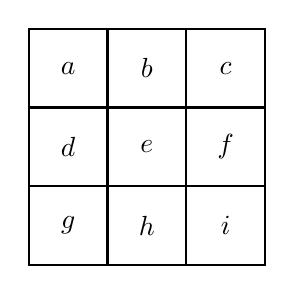
\begin{tikzpicture}
  \draw[line cap=rect, thick]
  grid(3, 3)
  foreach \x [count=\xi] in {a,...,i}{%
    ({0.5+mod(\xi-1,3},{2.5-div(\xi-1,3}) node{$\x$}};
\end{tikzpicture}

% coordinates
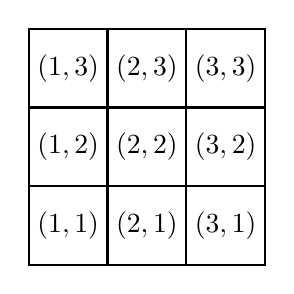
\begin{tikzpicture}
  \draw[line cap=rect, thick] grid(3, 3);
  \node at(0+0.5,0+0.5){$(1,1)$};
  \node at(1+0.5,0+0.5){$(2,1)$};
  \node at(2+0.5,0+0.5){$(3,1)$};
  \node at(0+0.5,1+0.5){$(1,2)$};
  \node at(1+0.5,1+0.5){$(2,2)$};
  \node at(2+0.5,1+0.5){$(3,2)$};
  \node at(0+0.5,2+0.5){$(1,3)$};
  \node at(1+0.5,2+0.5){$(2,3)$};
  \node at(2+0.5,2+0.5){$(3,3)$};
\end{tikzpicture}

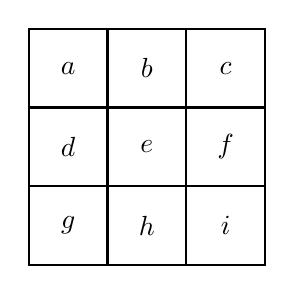
\begin{tikzpicture}
  \draw[line cap=rect, thick] grid(3, 3);
  \node at(0+0.5,2+0.5){$a$};
  \node at(1+0.5,2+0.5){$b$};
  \node at(2+0.5,2+0.5){$c$};
  \node at(0+0.5,1+0.5){$d$};
  \node at(1+0.5,1+0.5){$e$};
  \node at(2+0.5,1+0.5){$f$};
  \node at(0+0.5,0+0.5){$g$};
  \node at(1+0.5,0+0.5){$h$};
  \node at(2+0.5,0+0.5){$i$};
\end{tikzpicture}

\end{document}
